\section{问题四：考虑失水收缩的烘干时长}
\label{sec:q4}

\subsection{模型的建立：移动边界与坐标系选择}
\label{sec:q4model}

问题四要求考虑药材因失水而发生的尺寸变化，经验公式改用附录 4。由附件 2，药材半径由 $2.000$~cm 收缩到末值 $1.198$~cm，即\textbf{半径减少约 $40\%$}；而附件 2 只给出半径，未给出长度与体积的变化。因此本问首先要确定``失水如何改变形状''这一题目未明确给出的几何关系。

\subsubsection{几何假设与收缩运动学}

按假设 A10，本文取\textbf{长度不变}、收缩在径向\textbf{均匀}发生：同一物质壳层按同一比例缩放，即半径为 ${\rpos}_0$ 的初始物质点在任何时刻满足

\begin{equation}
\rpos({\rpos}_0,\t)=\frac{\R(\t)}{\Rzero}\,{\rpos}_0 .
\label{eq:kinematics}
\end{equation}

``长度不变''的依据是控制方程按\textbf{单位轴向长度}写出、$\Llen$ 不进入任何一项；代价是若长度按同一比例缩短，药材体积将只剩 $21.5\%$（而非固定长度假设下的 $35.9\%$），而附件 2 的数据\textbf{无法区分这两种情形}——这是本问最大的几何不确定性。

对式\eqref{eq:kinematics} 求时间导数，得到材料点的径向速度

\begin{equation}
v(\rpos,\t)=\left.\frac{\partial \rpos}{\partial \t}\right|_{{\rpos}_0}
=\frac{\dot \R}{\Rzero}{\rpos}_0=\frac{\dot \R}{\R}\,\rpos=\xi\dot \R,
\qquad \xi:=\frac{\rpos}{\R(\t)} .
\label{eq:materialvelocity}
\end{equation}

\subsubsection{干物质守恒与干基表观密度}

单位\textbf{当前}体积内的干物质质量为 $\rho_d(\t)$。由式\eqref{eq:kinematics}，半径 $\R$ 的圆柱内干物质质量正比于 ${\R}^2$，而干物质总量守恒，故

\begin{equation}
\rho_d(\t)\R(\t)^2=\rho_d(0){\Rzero}^2
\quad\Longrightarrow\quad
\rho_d(\t)=\rho_d(0)\left(\frac{\Rzero}{\R(\t)}\right)^2 .
\label{eq:rhod}
\end{equation}
即\textbf{材料被压缩，干基表观密度随半径的平方反比增大}。该关系可用干物质连续性方程自洽检验（径向均匀收缩时 $\partial\rho_d/\partial\rpos=0$）：

\begin{equation}
\frac{\partial \rho_d}{\partial \t}+\frac{1}{\rpos}\frac{\partial(\rpos\rho_d v)}{\partial \rpos}
=-\frac{2\rho_d\dot \R}{\R}+\frac{1}{\rpos}\frac{\partial}{\partial \rpos}\left(\rho_d\frac{{\rpos}^2\dot \R}{\R}\right)
=-\frac{2\rho_d\dot \R}{\R}+\frac{2\rho_d\dot \R}{\R}=0 .
\label{eq:dmcheck}
\end{equation}

\subsubsection{固定坐标下的水分守恒方程}

以干基含水率写水分守恒：单位体积内的水质量为 $\rho_d\C$，相对材料运动的扩散通量为 $-\rho_d\Ddiff\,\partial_\rpos\C$，故

\begin{equation}
\frac{\partial(\rho_d\C)}{\partial \t}
+\frac{1}{\rpos}\frac{\partial(\rpos\rho_d\C v)}{\partial \rpos}
=\frac{1}{\rpos}\frac{\partial}{\partial \rpos}\left(\rpos\rho_d\Ddiff\frac{\partial \C}{\partial \rpos}\right).
\label{eq:fixedframe}
\end{equation}
将左端展开（注意 $\rho_d$ 与 $\rpos$ 无关）：

\begin{equation}
\rho_d\frac{\partial \C}{\partial \t}
+\C\underbrace{\left(\frac{\partial\rho_d}{\partial \t}+\frac{\rho_d}{\rpos}\frac{\partial(\rpos v)}{\partial \rpos}\right)}_{=\,0\ \text{（式}\eqref{eq:dmcheck}\text{）}}
+\rho_d v\frac{\partial \C}{\partial \rpos}
=\frac{1}{\rpos}\frac{\partial}{\partial \rpos}\left(\rpos\rho_d\Ddiff\frac{\partial \C}{\partial \rpos}\right).
\end{equation}
两端约去 $\rho_d$ 后得到\textbf{固定物理坐标下的方程}

\begin{equation}
\frac{\partial \C}{\partial \t}+v\frac{\partial \C}{\partial \rpos}
=\frac{1}{\rpos}\frac{\partial}{\partial \rpos}\left(\rpos\Ddiff\frac{\partial \C}{\partial \rpos}\right).
\label{eq:euler}
\end{equation}
注意此时\textbf{必须保留}对流项 $v\,\partial_\rpos\C$：它来自材料本身的运动，是坐标原点不动带来的表观输运。

\subsubsection{材料坐标变换与严格相消}
\label{sec:cancellation}

若直接在式\eqref{eq:euler} 上求解，就必须处理随时间移动的边界 $\R(\t)$，并解决对流项带来的 CFL 限制。本文改为引入\textbf{材料坐标} $\xi=\rpos/\R(\t)\in[0,1]$，把移动域映射到固定域。由链式法则

\begin{equation}
\left.\frac{\partial}{\partial \rpos}\right|_{\t}=\frac{1}{\R}\left.\frac{\partial}{\partial \xi}\right|_{\t},
\qquad
\left.\frac{\partial \xi}{\partial \t}\right|_{\rpos}=-\frac{\rpos\dot \R}{{\R}^2}=-\frac{\xi\dot \R}{\R},
\end{equation}

\begin{equation}
\left.\frac{\partial}{\partial \t}\right|_{\rpos}
=\left.\frac{\partial}{\partial \t}\right|_{\xi}+\left.\frac{\partial \xi}{\partial \t}\right|_{\rpos}\frac{\partial}{\partial \xi}
=\left.\frac{\partial}{\partial \t}\right|_{\xi}-\frac{\xi\dot \R}{\R}\frac{\partial}{\partial \xi}.
\label{eq:chainrule}
\end{equation}
把式\eqref{eq:chainrule} 与式\eqref{eq:materialvelocity} 代入式\eqref{eq:euler} 的左端，得到本问推导中最关键的一步：

\begin{equation}
\underbrace{\left.\frac{\partial \C}{\partial \t}\right|_{\rpos}}_{=\,{\C}_\t|_\xi-\frac{\xi\dot \R}{\R}{\C}_\xi}
+v\underbrace{\frac{\partial \C}{\partial \rpos}}_{=\,{\C}_\xi/\R}
={\C}_\t\big|_\xi-\frac{\xi\dot \R}{\R}{\C}_\xi+(\xi\dot \R)\frac{{\C}_\xi}{\R}
={\C}_\t\big|_\xi .
\label{eq:cancel}
\end{equation}

\textbf{坐标变换引入的输运项 $-\frac{\xi\dot \R}{\R}{\C}_\xi$ 与材料速度带来的对流项 $+\frac{\xi\dot \R}{\R}{\C}_\xi$ 大小相等、符号相反，恰好严格相消}。换言之，物质导数就等于固定 $\xi$ 的偏导数：

\begin{equation}
\frac{\mathrm{D}\C}{\mathrm{D}\t}
:=\left.\frac{\partial \C}{\partial \t}\right|_{\rpos}+v\frac{\partial \C}{\partial \rpos}
=\left.\frac{\partial \C}{\partial \t}\right|_{\xi}.
\end{equation}
这不是巧合：由式\eqref{eq:kinematics}，$\xi$ 被材料速度平流（$\xi_\t+v\xi_\rpos=-\frac{\xi\dot \R}{\R}+\xi\dot \R\cdot\frac1{\R}=0$），因此固定 $\xi$ 的点始终跟踪同一团材料，$\xi$ 是\textbf{材料标签}而非纯数学技巧。

右端的扩散算子作同样变换：

\begin{equation}
\frac{1}{\rpos}\frac{\partial}{\partial \rpos}\left(\rpos\Ddiff\frac{\partial \C}{\partial \rpos}\right)
=\frac{1}{{\R}^2\xi}\frac{\partial}{\partial \xi}\left(\xi\Ddiff\frac{\partial \C}{\partial \xi}\right).
\end{equation}

\subsubsection{变换后的方程组与表面条件}

综合以上结果，得到问题四在\textbf{固定计算域 $\xi\in[0,1]$} 上的控制方程组：

\begin{equation}
\boxed{\
\left.\frac{\partial \C}{\partial \t}\right|_{\xi}=\frac{1}{{\R}^2(\t)\,\xi}\frac{\partial}{\partial \xi}\left(\xi\,\Ddiff\frac{\partial \C}{\partial \xi}\right),
\qquad
\rho\cp\left.\frac{\partial \T}{\partial \t}\right|_{\xi}=\frac{1}{{\R}^2(\t)\,\xi}\frac{\partial}{\partial \xi}\left(\xi\,\kcond\frac{\partial \T}{\partial \xi}\right)
\ }
\label{eq:q4system}
\end{equation}
其中物性取附录 4（$\rho=760+90\C$、$\cp=1850+2150\wfrac$、$\kcond=0.12+0.20\wfrac$、$\Ddiff=4.2\times10^{-4}e^{-0.30/\C}e^{-3850/\T}$，$\wfrac=\C/(1+\C)$，$\T$ 用开尔文）。\textbf{与前三问相比，方程组的形式完全相同，只多出一个 $1/{\R}^2(\t)$ 的整体因子，且不含任何对流项。}物理含义是：$\xi$ 坐标下所有长度都按 $\R(\t)$ 缩放，扩散算子只被 $1/{\R}^2$ 加速；由于 $\R$ 减小，\textbf{特征扩散时间 ${\R}^2/\Ddiff$ 随之缩短}。

表面条件（$\xi=1$）由 $\partial_\rpos={\R}^{-1}\partial_\xi$ 与式\eqref{eq:robin} 给出：

\begin{equation}
\Ddiff\left.\frac{\partial \C}{\partial \xi}\right|_{\xi=1}=-\R\,\hmass\,({\C}_s-\Cinf),
\qquad
\kcond\left.\frac{\partial \T}{\partial \xi}\right|_{\xi=1}=\R\,\hconv\,(\Tinf-{\T}_s).
\label{eq:q4bc}
\end{equation}
系数中多出的 $\R$ 是把``对 $\rpos$ 的梯度''换成``对 $\xi$ 的梯度''带来的几何因子（梯度被拉长了 $1/\R$ 倍），它与方程中的 $1/{\R}^2$ 一起决定传热与失水的速率。轴心条件仍为 $\partial_\xi\T=\partial_\xi\C=0$；初值仍为式\eqref{eq:initial}（$\t=0$ 时 $\R(0)=\Rzero$，故与前三问逐字相同）。

\subsubsection{必须避免的一个错误：不得再加对流项}

式\eqref{eq:cancel} 的相消是\textbf{逐项}完成的：链式法则产生 $-\frac{\xi\dot \R}{\R}{\C}_\xi$，材料速度产生 $+\frac{\xi\dot \R}{\R}{\C}_\xi$。因此\textbf{在式\eqref{eq:q4system} 上再次添加 $\frac{\xi\dot \R}{\R}{\C}_\xi$ 这一项是重复计入}，等价于凭空引入一个不存在的相对流动，会系统性地偏移干燥速率。

只有在下列情形才需要那一项：(i) 在\textbf{固定物理坐标} $\rpos$ 上求解而边界在动（即直接用式\eqref{eq:euler}）；(ii) 假设\textbf{非均匀收缩}，此时存在径向的相对材料速度，式\eqref{eq:dmcheck} 中的相消不再成立；(iii) 用不随材料缩放的固定网格做离散。本文三种情形都不是：网格节点是材料点，故方程中不应出现对流项。判断方法是问一句``\textbf{这个模型的网格节点是材料点还是空间点}''。

\subsubsection{退化检验}

取 $\R\equiv\Rzero$（即 $\dot \R=0$），式\eqref{eq:q4system} 退化为固定域上的方程 ${\C}_\t=(\xi\Ddiff{\C}_\xi)_\xi/({\Rzero}^2\xi)$，配合 $\Ddiff{\C}_\xi|_{\xi=1}=-\Rzero\hmass({\C}_s-\Cinf)$，与前三问在缩放坐标下的形式完全一致。程序层面做了这一检验：把附件 2 的半径序列全部置为 $\Rzero$ 后，材料坐标模式与固定半径模式的右端函数\textbf{逐位相同}（差值严格为 $0$），既验证了式\eqref{eq:cancel} 的相消，也验证了实现没有多加或少加对流项。

\subsection{模型的求解}
\label{sec:q4solve}

\subsubsection{固定材料坐标网格上的离散}

由于 $\xi$ 是材料坐标（式\eqref{eq:kinematics}），在 $\xi$ 网格上离散时式\eqref{eq:q4system} 的算子结构不随时间改变，因此仍使用第~\ref{sec:mesh} 节的表面二次加密网格（式\eqref{eq:gradedmesh}）与节点中心有限体积格式，只是每个时刻都要按当时的 $\R(\t)$ 更新方程中的 $1/{\R}^2$ 因子与界面通量：

\begin{equation}
F^C_{i+1/2}=\xi_{i+1/2}\,{\Ddiff}_{i+1/2}\frac{{\C}_{i+1}-{\C}_i}{\Delta\xi_i},
\qquad
F^T_{i+1/2}=\xi_{i+1/2}\,{\kcond}_{i+1/2}\frac{{\T}_{i+1}-{\T}_i}{\Delta\xi_i},
\end{equation}
\begin{equation}
\frac{\mathrm{d}{\C}_i}{\mathrm{d}\t}=\frac{F^C_{i+1/2}-F^C_{i-1/2}}{{\R}^2V_i},
\qquad
\frac{\mathrm{d}{\T}_i}{\mathrm{d}\t}=\frac{F^T_{i+1/2}-F^T_{i-1/2}}{{\R}^2V_i\rho_i{\cp}_i},
\qquad
F^C_{\Nr-1/2}=-\R\hmass({\C}_s-\Cinf),\quad F^T_{\Nr-1/2}=-\R\hconv({\T}_s-\Tinf).
\end{equation}

时间积分沿用第~\ref{sec:time} 节的 BDF 方法，环境条件按式\eqref{eq:interp} 插值并在附件 1 的每个测量节点重启；半径 $\R(\t)$ 由附件 2 分段线性插值，且在 $\t$ 超出附件 2 的覆盖范围时直接报错而\textbf{不做外推}（本问的终点 $50.82$~h 落在数据覆盖的 $72$~h 之内，不需要外推）。此外，由于 $1/{\R}^2$ 使方程的系数随时间变化，右端函数中的 $\R$ 与 $\dot\R$ 无关（$\dot\R$ 不进入方程，见第~\ref{sec:cancellation} 节），故附件 2 的分段线性插值在节点处的导数跳变\textbf{不构成任何数值困难}——这是材料坐标建模除实现简单之外的第二个实质好处。

\subsubsection{交付映射}

导出阶段的关键是``内部解在材料坐标上、交付网格在物理坐标上''。对第 $j$ 个输出时刻，先由附件 2 得到 ${\R}_j=\R(t_j)$，把内部节点映射为物理位置 ${\rpos}_{i,j}=\xi_i{\R}_j$，再把该时刻的含水率场插值到题目要求的固定物理位置 $0,0.1,\ldots,1.9$~cm 上；落在当时药材之外的列\textbf{留空}。交付文件的末列``药材表面''取 $\xi=1$ 节点的值，它恒为有效值，与域外留空无关。以交付文件末行（$t=183000$~s，$\R=1.2000$~cm）为例：$0$~cm 与 $1.2$~cm 列的含水率为 $0.1500$ 与 $0.0525$~kg/kg，$1.3\sim1.9$~cm 共 $7$ 列留空，末列``药材表面''与 $1.2$~cm 列相同（此时两者是同一物理位置）——这一自洽性可直接用于检验交付文件的正确性。

\subsection{结果与分析}
\label{sec:q4result}

\subsubsection{烘干时长}

\begin{equation}
\boxed{\ \tend^{(\text{问题 4})}=\QFourEventS~\mathrm{s}=\QFourEventH~\mathrm{h}\ }
\end{equation}

即考虑失水收缩后，烘干时长为 \textbf{\QFourEventH~h}。事件时刻的药材半径为 $\R=\QFourEventR$~cm（由初始 $2.0000$~cm 收缩 \QFourShrinkPct\%），表面含水率为 \QFourSurfaceEnd~kg/kg，温度场仍为全场 $323.315$~K。交付文件 \texttt{result4.xlsx} 写到 \QFourLastRowS~s（即 \QFourEventH~h 之后的第一个 $60$~s 整行）。按题目表 6 格式整理的结果见表~\ref{tab:q4-moisture}。

\geninput{tab/q4_moist}{表 6 由 \texttt{make tables} 从 \texttt{results/tables/q4\\_moist.csv} 生成；末列为当时的药材表面位置。}

\subsubsection{半径收缩的结构}

\begin{figure}[!ht]
  \centering
  \IfFileExists{figs/fig-q4-shrink.pdf}{%
    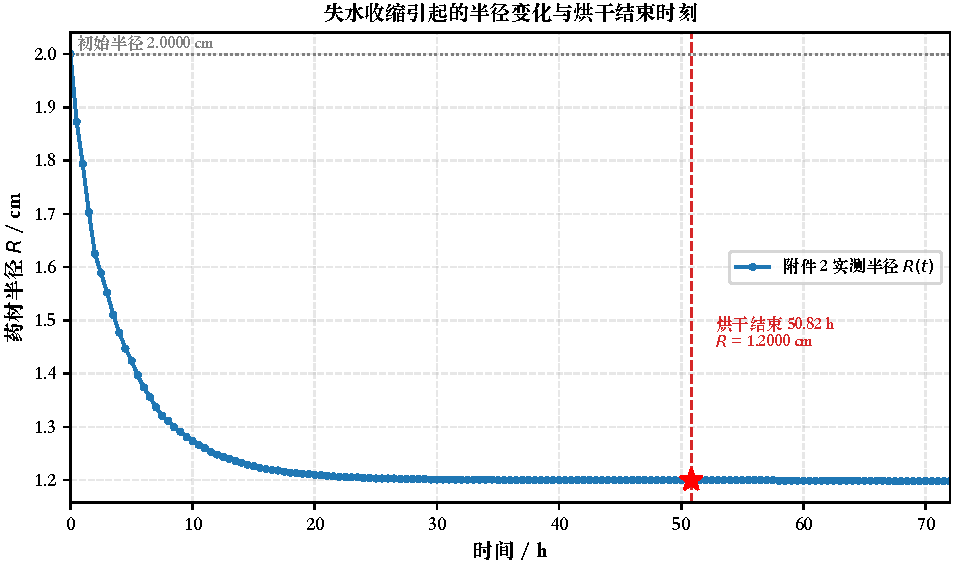
\includegraphics[width=0.45\linewidth]{figs/fig-q4-shrink.pdf}%
  }{%
    \instruction{【插图缺失】未找到 \texttt{figs/fig-q4-shrink.pdf}，请先运行 \texttt{make figs}。}%
  }
  \caption{附件 2 给出的药材半径随时间的收缩过程与烘干结束时刻（红星标出结束时刻的半径）}
  \label{fig:q4-shrink}
\end{figure}

图~\ref{fig:q4-shrink} 显示附件 2 的半径序列有三个特征。第一，\textbf{收缩主要发生在前 $3$~h}：半径由 $2.000$~cm 迅速降到约 $1.51$~cm，此后速率明显变缓；第二，$18$~h 之后半径进入近似台阶状的小幅下降，$35.0\sim57.5$~h 之间保持 $1.2000$~cm 不变；第三，\textbf{本问的烘干结束时刻 $50.82$~h 恰好落在这一平台内部}。第三点有重要的实务含义：\textbf{答案不依赖半径数据在结束时刻附近的插值细节}（该区间内 $\R$ 是常数），因此半径测量的小幅波动不会影响报出的烘干时长。同时这也说明``半径不再变化''只在小数点后两位成立：到附件 2 的末值 $1.1980$~cm 还要再降 $0.002$~cm，且发生在 $67$~h 之后。

\subsubsection{两个相反效应的分离：三个算例的对照}

由于问题三与问题四\textbf{同时}改变了物性集（附录 3 $\to$ 附录 4）与几何（固定半径 $\to$ 收缩半径），直接比较 $57.17$~h 与 $50.82$~h 无法说明收缩的作用。为此本文构造第三个算例：\textbf{同用附录 4 物性、但半径固定为 $\Rzero$}，从而把两个效应分离开。三个算例的结果如下：

\begin{table}[!ht]
  \centering
  \caption{分离参数集效应与几何效应的三个算例（B 为本文构造的对照算例，不产出交付文件）}
  \label{tab:three-cases}
  \scriptsize
  \begin{tabular}{ccccc}
    \toprule
    算例 & 物性 & 半径 & 烘干时长 / h & 用途 \\
    \midrule
    A（问题三） & 附录 3 & $\Rzero$ 固定 & $57.1694$ & 基准 \\
    B（对照算例） & 附录 4 & $\Rzero$ 固定 & \QFourFixedRadiusH & 与 A 比较即得参数集效应 \\
    C（问题四） & 附录 4 & $2.000\to\QFourEventR$~cm & \QFourEventH & 与 B 比较即得收缩效应 \\
    \bottomrule
  \end{tabular}
\end{table}

\begin{itemize}
  \item \textbf{参数集效应（A$\to$B）}：在固定几何下把物性换成附录 4 后，烘干时长由 $57.17$~h 增大到 \QFourFixedRadiusH~h，即\textbf{变慢 $2.26$ 倍}。原因是附录 4 的扩散系数前因子比附录 3 小约 $5.7$ 倍（$4.2\times10^{-4}$ 对 $2.4\times10^{-3}$），而 $\C$ 的指数由 $-0.45/\C$ 变为 $-0.30/\C$，二者共同使扩散变慢。
  \item \textbf{收缩效应（B$\to$C）}：在\textbf{同一物性集}下把半径由固定改为按附件 2 收缩，烘干时长由 \QFourFixedRadiusH~h 降到 \QFourEventH~h，即\textbf{缩短 \QFourShrinkEffectPct\%}。
  \item \textbf{净效应（A$\to$C）}：两者叠加后 $57.17$~h 变为 \QFourEventH~h，缩短 \QFourNetEffectPct\%。\textbf{这个数字是两个方向不同效应的净值，单独引用会得到误导性的结论。}
\end{itemize}

\genfig[0.70\linewidth]{figs/fig-param-comparison.pdf}{三个算例的烘干时长对照。黑色实线为问题三（附录 3、固定半径）的含水率历程，另外两条竖线分别标出对照算例（附录 4、固定半径）与问题四（附录 4、收缩半径）的终点时刻}{fig:param-comparison}

\subsubsection{为什么收缩在本模型下使干燥加快}

直觉上``半径减小 $\Rightarrow$ 水分逸出面积减小 $\Rightarrow$ 干燥变慢''，与算例 B$\to$C 的结果相反。要弄清哪一效应占优，必须把两个效应换算到同一度量上。对式\eqref{eq:q4system} 沿断面按材料测度积分（$\int_0^1(\cdot)\,\xi\,\mathrm{d}\xi$，对应离散的 $\sum_iV_i{\C}_i$），并代入表面条件式\eqref{eq:q4bc}：

\begin{equation}
\frac{\mathrm{d}}{\mathrm{d}\t}\int_0^1\C\,\xi\,\mathrm{d}\xi
=\frac{1}{{\R}^2}\left[\xi\Ddiff{\C}_\xi\right]_{\xi=0}^{\xi=1}
=\frac{\Ddiff{\C}_\xi(1)}{{\R}^2}
=-\frac{\hmass({\C}_s-\Cinf)}{\R}.
\label{eq:lossrate}
\end{equation}
即单位材料测度的失水速率为 $\hmass({\C}_s-\Cinf)/\R$。再换成单位长度药材的失水质量：由式\eqref{eq:rhod}，$\rho_d(\t){\R}^2\equiv\text{const}$，故

\begin{equation}
W=\rho_d{\R}^2\cdot2\pi\int_0^1\C\xi\,\mathrm{d}\xi
\quad\Longrightarrow\quad
\frac{\mathrm{d}W}{\mathrm{d}\t}=-2\pi\underbrace{\R}_{\text{面积因子}}\underbrace{\rho_d}_{\propto\,{\R}^{-2}}\hmass({\C}_s-\Cinf).
\label{eq:twochannels}
\end{equation}

于是两条通道各自的量纲因子为：\textbf{表面积通道}正比于 $\R$（半径减小使逸出面积变小，趋于$\cdot$变慢）；\textbf{干基密度通道}正比于 ${\R}^{-2}$（材料被压实，单位体积内的水量随半径平方反比增大，趋于变快）；两者相乘后\textbf{净表面项正比于 ${\R}^{-1}$，即趋于变快}。与此同时，\textbf{内部再分布的时间尺度正比于 ${\R}^2/\Ddiff$}，半径减小同样使它变快。

因此在本模型所采用的边界闭合下，\textbf{``面积减小''这一条并没有表现为净减速}：干基表观密度随收缩上升（式\eqref{eq:rhod}）把面积因子完全抵消并超过，两个通道都指向变快。定量地看，算例 B$\to$C 的时长比为 $50.8242/129.0926=0.394$，而 $({\R}_{\text{end}}/\Rzero)^2=(1.2000/2.0000)^2=0.360$，二者同量级；这与``内部扩散控制下时间尺度正比于 ${\R}^2/\Ddiff$''的判断一致，也说明\textbf{路径缩短占主导}。

需要明确的是，这一结论\textbf{依赖于表面传质的闭合形式}（假设 A7）。若改用``水蒸气通量正比于表面积''的另一种闭合，面积减小的效应会重新出现，结论可能改变。本文如实陈述本模型下的结论，并在第~\ref{sec:limitations} 节把它列为一项结构性限制，而不通过``在材料坐标方程里再加一个对流项''的方式人为制造``面积效应''（第~\ref{sec:cancellation} 节已论证那是重复计入）。

\genfig[0.60\linewidth]{figs/fig4-C-profiles.pdf}{含收缩时水分浓度沿材料坐标 $\xi=\rpos/\R(\t)$ 的分布（问题四）}{fig:q4C}
\genfig[0.60\linewidth]{figs/fig4-C-history.pdf}{不同径向位置的水分浓度随时间的变化（问题四，位置按固定物理距离取值）}{fig:q4Chistory}

\subsubsection{与问题三的对比}

图~\ref{fig:q4C}、图~\ref{fig:q4Chistory} 给出问题四的剖面与历程。与问题三（图~\ref{fig:q3C}、图~\ref{fig:q3Chistory}）相比有三点值得注意。

第一，\textbf{干燥曲线的形状相同、时间轴被压缩}。问题四的剖面同样经历``表层先降—前沿内推—整体趋平''三段，只是各段的时间尺度按 ${\R}^2$ 成比例缩短：问题三中表面在 $12$~h 才降到 $0.1639$~kg/kg，问题四中 $12$~h 时表面已降到 $0.1667$~kg/kg（此时半径已收缩到 $1.3740$~cm，而问题三在同一时刻的半径仍是 $2.0$~cm）；问题三中轴心在 $36$~h 为 $0.1854$~kg/kg，问题四中同一时刻为 $0.1921$~kg/kg，剖面的相对形状也与问题三基本一致。

第二，\textbf{交付表在形态上与前三问不同}。表~\ref{tab:q4-moisture} 的 $1.5$~cm 列在各时刻\textbf{均留空}：因为 $\t=6$~h 时半径已收缩到 $1.3740$~cm，固定位置 $1.5$~cm 落在药材之外。这不是数据缺失，而是``交付位置是固定物理位置、药材却在收缩''的必然结果，也是题目把末列改为``药材表面''的原因。

第三，\textbf{末期的剖面更平坦}。结束时刻问题四的中心与表面含水率分别为 $0.15$ 与 $0.0525$~kg/kg（差 $0.0975$），与问题三几乎相同；但由于此时药材只有 $1.2$~cm 半径，同样的绝对差值对应的\textbf{相对梯度更大}，这说明收缩后期内部水分向外补充的``路程''虽短，含水率的相对落差并未减小。
